

\section{OpticalElement: \textquotedbl{}MICADO\_SPEC\textquotedbl{}%
  \label{opticalelement-micado-spec}%
}

\textbf{Element}: instrument

\textbf{Alias}: INST

\textbf{Description}: additional effects for the spectroscopy mode


\subsection{Global properties%
  \label{global-properties}%
}

\begin{quote}
\begin{alltt}
\begin{lstlisting}[frame=single]
 pixel_scale : 0.004
 plate_scale : 0.2666666667
element_name : MICADO_SPEC
\end{lstlisting}
\end{alltt}
\end{quote}


\subsection{Effects%
  \label{effects}%
}

Summary of Effects included in this optical element:

\setlength{\DUtablewidth}{\linewidth}
\begin{longtable*}[c]{|p{0.141\DUtablewidth}|p{0.323\DUtablewidth}|p{0.209\DUtablewidth}|p{0.107\DUtablewidth}|p{0.175\DUtablewidth}|}
\hline
\textbf{%
element
} & \textbf{%
name
} & \textbf{%
class
} & \textbf{%
included
} & \textbf{%
z\_orders
} \\
\hline
\endfirsthead
\hline
\textbf{%
element
} & \textbf{%
name
} & \textbf{%
class
} & \textbf{%
included
} & \textbf{%
z\_orders
} \\
\hline
\endhead
\multicolumn{5}{c}{\hfill ... continued on next page} \\
\endfoot
\endlastfoot

MICADO\_SPEC
 & 
spec\_mode\_optics
 & 
SurfaceList
 & 
True
 & 
{[}20, 120, 520{]}
 \\
\hline

MICADO\_SPEC
 & 
spectroscopic\_slit\_aperture
 & 
ApertureMask
 & 
True
 & 
{[}80, 280, 380{]}
 \\
\hline

MICADO\_SPEC
 & 
micado\_spectral\_traces
 & 
SpectralTraceList
 & 
True
 & 
{[}70, 270{]}
 \\
\hline
\end{longtable*}
\label{tbl-micado-spec}


\subsubsection{SurfaceList: \textquotedbl{}spec\_mode\_optics\textquotedbl{}%
  \label{surfacelist-spec-mode-optics}%
}

\textbf{Included by default}: \texttt{True}

\textbf{File Description}: list of extra mirrors needed for the spectroscopy mode

\textbf{Class Description}: <no docstring>

\textbf{Changes}:

\begin{itemize}
\item 2019-01-28 (KL) Changed column names and added units to header

\item 2019-07-10 (KL) Shortened the list to only the swappable gratings
\end{itemize}


\paragraph{Data%
  \label{data}%
}

\begin{figure}[H]
\noindent\makebox[\linewidth][c]{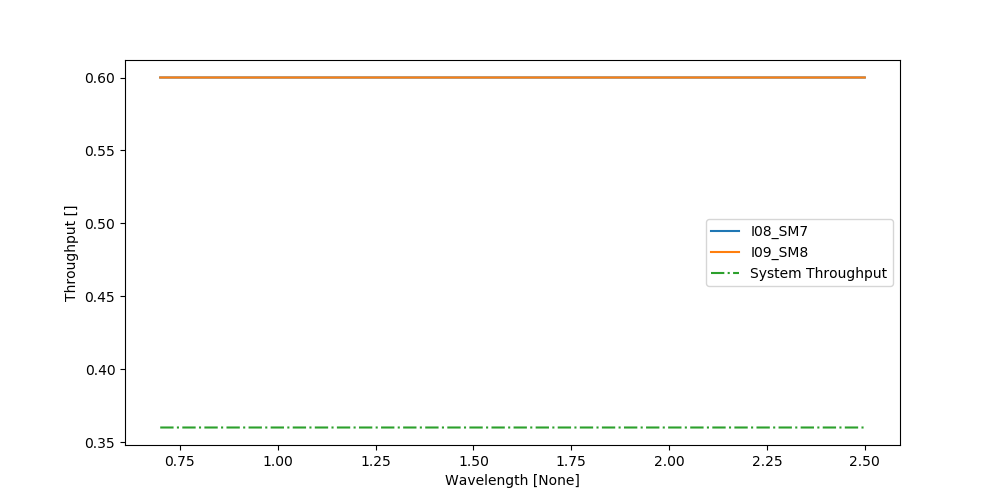
\includegraphics{spec_mode_optics.png}}\phantomsection\label{fig-spec-mode-optics}
\end{figure}

\setlength{\DUtablewidth}{\linewidth}
\begin{longtable*}[c]{|p{0.098\DUtablewidth}|p{0.075\DUtablewidth}|p{0.075\DUtablewidth}|p{0.075\DUtablewidth}|p{0.145\DUtablewidth}|p{0.133\DUtablewidth}|p{0.191\DUtablewidth}|}
\hline
\textbf{%
name
} & \textbf{%
outer
} & \textbf{%
inner
} & \textbf{%
angle
} & \textbf{%
temperature
} & \textbf{%
action
} & \textbf{%
filename
} \\
\hline
\endfirsthead
\hline
\textbf{%
name
} & \textbf{%
outer
} & \textbf{%
inner
} & \textbf{%
angle
} & \textbf{%
temperature
} & \textbf{%
action
} & \textbf{%
filename
} \\
\hline
\endhead
\multicolumn{7}{c}{\hfill ... continued on next page} \\
\endfoot
\endlastfoot

I08\_SM7
 & 
0.2
 & 
0.0
 & 
0
 & 
-190
 & 
reflection
 & 
TER\_grating.dat
 \\
\hline

I09\_SM8
 & 
0.2
 & 
0.0
 & 
0
 & 
-190
 & 
reflection
 & 
TER\_grating.dat
 \\
\hline
\end{longtable*}
\label{tbl-spec-mode-optics}


\paragraph{Meta-data%
  \label{meta-data}%
}

\begin{quote}
\begin{alltt}
\begin{lstlisting}[frame=single]
            filename : LIST_MICADO_mirrors_spec.dat
                name : spec_mode_optics
         pixel_scale : 0.004
         plate_scale : 0.2666666667
        element_name : MICADO_SPEC
              author : Kieran Leschinski
              source : Ric's SPIE 2018 PPT presentation
        date_created : 2018-11-19
       date_modified : 2019-07-10
              status : Design, pre PDR list of swappable optics for spectroscopy
                type : mirror:list
               ETYPE : SURFLIST
                EDIM : 1
          outer_unit : m
          inner_unit : m
          angle_unit : degree
    temperature_unit : deg_C
             z_order : [20, 120, 520]
             include : True
        ignore_wings : False
            wave_min : !SIM.spectral.wave_min
            wave_max : !SIM.spectral.wave_max
           wave_unit : !SIM.spectral.wave_unit
            wave_bin : !SIM.spectral.spectral_resolution
 report_plot_include : True
report_table_include : True
  minimum_throughput : !SIM.spectral.minimum_throughput
             etendue : !TEL.etendue
\end{lstlisting}
\end{alltt}
\end{quote}


\subsubsection{ApertureMask: \textquotedbl{}spectroscopic\_slit\_aperture\textquotedbl{}%
  \label{aperturemask-spectroscopic-slit-aperture}%
}

\textbf{Included by default}: \texttt{True}

\textbf{File Description}: Slit mask for the short, wide slit  (3 arcsec x 50 mas)

\textbf{Class Description}: Only provides the on-sky window coords of the Aperture

\textbf{Changes}:

\begin{itemize}
\item 2019-07-10 (KL) Created the file

\item 2020-03-24 (KL) Changed geometry to 3000x50mas
\end{itemize}


\paragraph{Data%
  \label{id1}%
}
\leavevmode
\setlength{\DUtablewidth}{\linewidth}
\begin{longtable*}[c]{|p{0.098\DUtablewidth}|p{0.098\DUtablewidth}|}
\hline
\textbf{%
x
} & \textbf{%
y
} \\
\hline
\endfirsthead
\hline
\textbf{%
x
} & \textbf{%
y
} \\
\hline
\endhead
\multicolumn{2}{c}{\hfill ... continued on next page} \\
\endfoot
\endlastfoot

-1.5000
 & 
-0.0250
 \\
\hline

1.5000
 & 
-0.0250
 \\
\hline

1.5000
 & 
0.0250
 \\
\hline

-1.5000
 & 
0.0250
 \\
\hline
\end{longtable*}
\label{tbl-spectroscopic-slit-aperture}


\paragraph{Meta-data%
  \label{id2}%
}

\begin{quote}
\begin{alltt}
\begin{lstlisting}[frame=single]
             filename : !OBS.slit_file
                 name : spectroscopic_slit_aperture
          pixel_scale : 0.004
          plate_scale : 0.2666666667
         element_name : MICADO_SPEC
               author : Kieran Leschinski
               source : My imagination
         date_created : 2019-07-10
        date_modified : 2019-07-10
               status : Guess - in the train on the way home from CM13
                 type : aperture:slit_geometry
               x_unit : arcsec
               y_unit : arcsec
              z_order : [80, 280, 380]
              include : True
              no_mask : True
                angle : 0
                shape : rect
       conserve_image : True
                   id : 0
  report_plot_include : False
 report_table_include : True
report_table_rounding : 4
\end{lstlisting}
\end{alltt}
\end{quote}


\subsubsection{<SpectralTraceList> \textquotedbl{}micado\_spectral\_traces\textquotedbl{} : 17 traces%
  \label{spectraltracelist-micado-spectral-traces-17-traces}%
}

\textbf{Included by default}: \texttt{True}

\textbf{File Description}: list of spectral order trace geometry on the focal plane

\textbf{Class Description}: List of spectral trace geometries for the detector plane

\textbf{Changes}:

\begin{itemize}
\item \end{itemize}


\paragraph{Data%
  \label{id3}%
}

\begin{figure}[H]
\noindent\makebox[\linewidth][c]{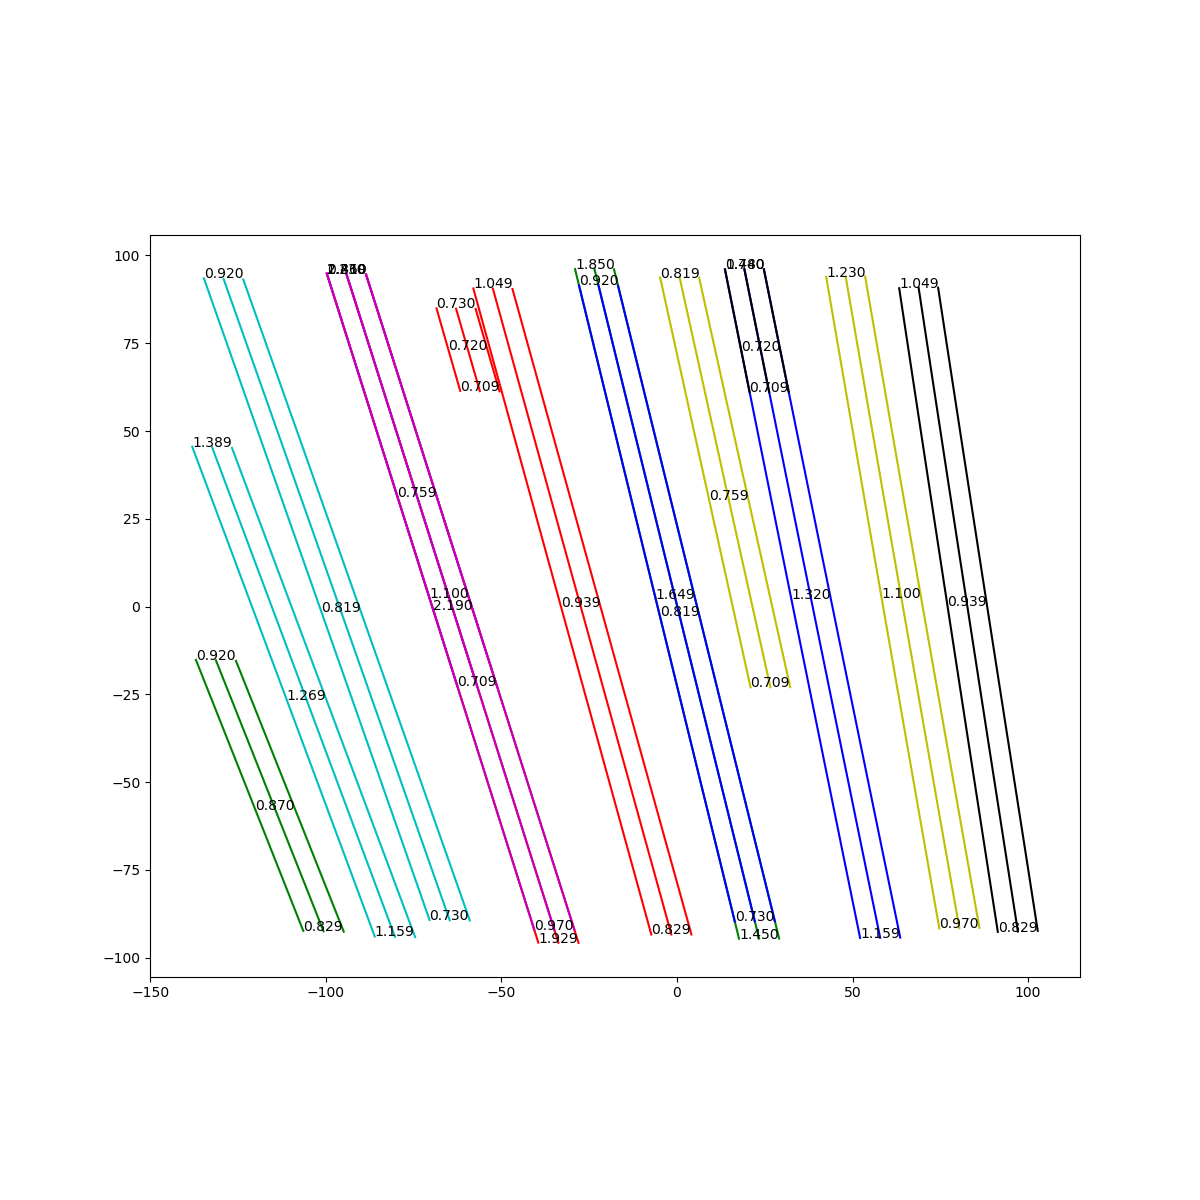
\includegraphics{micado_spectral_traces.png}}\phantomsection\label{fig-micado-spectral-traces}
\end{figure}


\paragraph{Meta-data%
  \label{id4}%
}

\begin{quote}
\begin{alltt}
\begin{lstlisting}[frame=single]
            filename : !OBS.trace_file
                name : micado_spectral_traces
         pixel_scale : 0.004
         plate_scale : 0.2666666667
        element_name : MICADO_SPEC
        wave_colname : lam
           s_colname : xi
    col_number_start : 1
       invalid_value : 0
              SIMPLE : True
              BITPIX : 8
               NAXIS : 0
              EXTEND : True
            FILETYPE : Spectral Layout Definition
              AUTHOR : Oliver Czoske
                DATE : 2018-09-16
              SOURCE : Frank Grupp
            ORIGDATE : 2018-06-29
              STATUS : Design PDR
                ECAT : 1
               EDATA : 2
            DESCRIPT : Maps spectral traces from long slit aperture to detector image plane
            DATE_CRE : 2018-06-29
            DATE_MOD : 2019-09-16
             HISTORY : 2019-09-16 : (KL) Added aperture-imagePlane table to EXT 1
             z_order : [70, 270]
             include : True
            wave_min : !SIM.spectral.wave_min
            wave_mid : !SIM.spectral.wave_mid
            wave_max : !SIM.spectral.wave_max
           x_colname : x
           y_colname : y
  center_on_wave_mid : False
               dwave : 0.002
 report_plot_include : True
report_table_include : False
\end{lstlisting}
\end{alltt}
\end{quote}
